

\title{Lab Report 02 - Local Features}
\author{
        Manuel Galliker  14-921-969 \\
                manuelga@student.ethz.ch
}
\date{\today}

\documentclass[12pt]{article}
\usepackage{graphicx}
\begin{document}
\maketitle


\section{Detection}
First the derivatives in x and y directions are calculated using conv2. afterwards the function imagusfilt was used to directly blur components of the local auto-correlation matrix. This function is then used to calculate the Harris respone function $C$ according to the given formulas. The Harris Response function is a computational less demanding way to ensure both eigenvalues of the harris response function are large. 
Therefore we can find the potential corner points by threshholding the Harris Response function for each point. 
Additionally we want to make sure that we only capture the points around the local maxima function. Otherwise all points close to the corner which fullfil the threshhold criteria will be recognized as corners. 
Therefore we combine the threshholds condition with a regional maxima condition using the imregionalmax function. 
This then results in an matrix of detected corner points. 
\vspace{5mm}
\newline
\begin{figure}[ht]
	\centering
	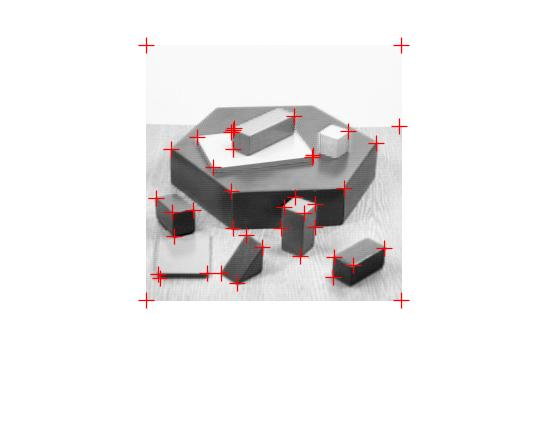
\includegraphics[width=0.9\textwidth]{corners_blocks.jpg}
	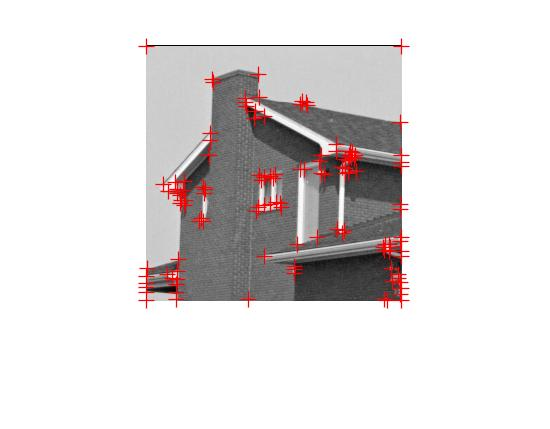
\includegraphics[width=0.9\textwidth]{corners_house.jpg}
	\caption{Detected Corners on blocks and house images}
	\label{fig1}
\end{figure}
\vspace{5mm}
\newline
By experimentation it was seen the changes in sigma and k didn't have a large effect on the quality of the corner detection. However the threshhold influenced the amout of detected corners in a strong was. It was tuned to include as many corners as possible before detecting points on edges as corners. 

The final choice of parameters was: 
$sigma =    1$
\vspace{5mm}
\newline
$k =    0.05$
\vspace{5mm}
\newline
$thresh = 0.00001$

\section{Description and Matching}

The algorithms were implemented as described in the exercise. 

\vspace{5mm}
\begin{figure}[ht]
	\centering
	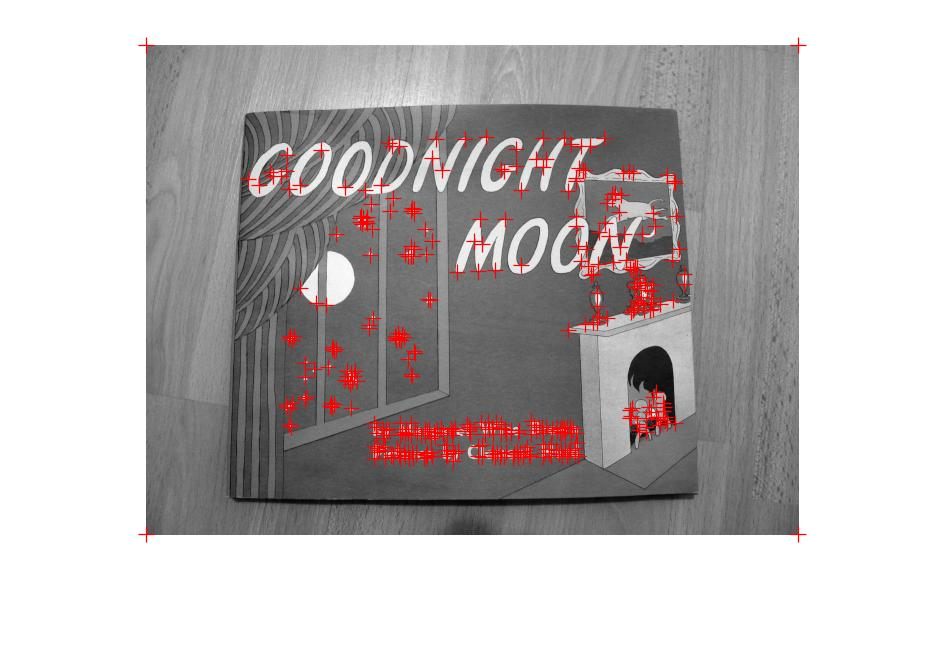
\includegraphics[width=0.9\textwidth]{20.jpg}
	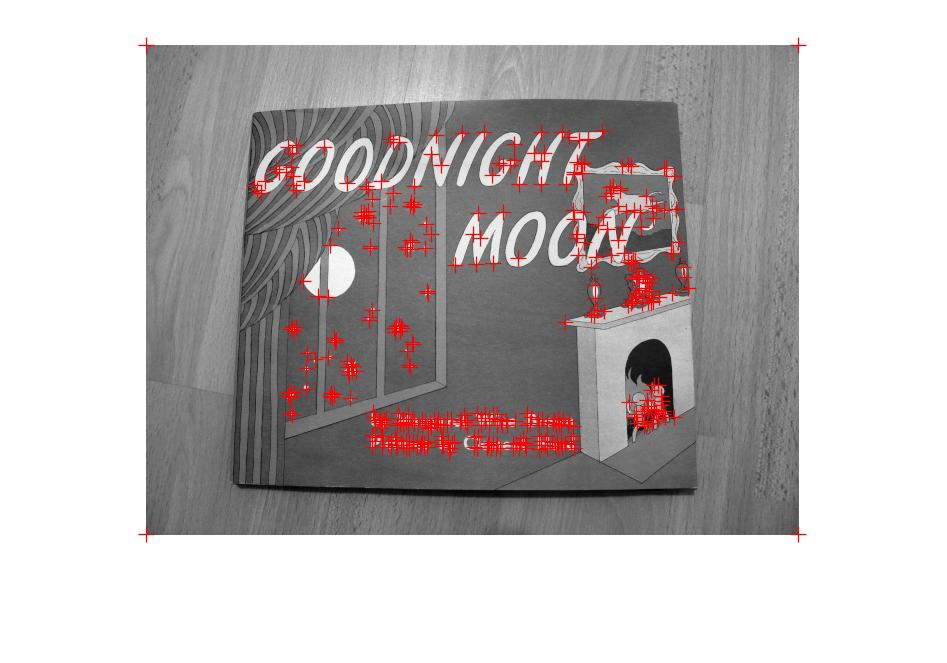
\includegraphics[width=0.9\textwidth]{21.jpg}
	\caption{Corner Detection}
	\label{fig1}
\end{figure}
\begin{figure}[ht]
	\centering
	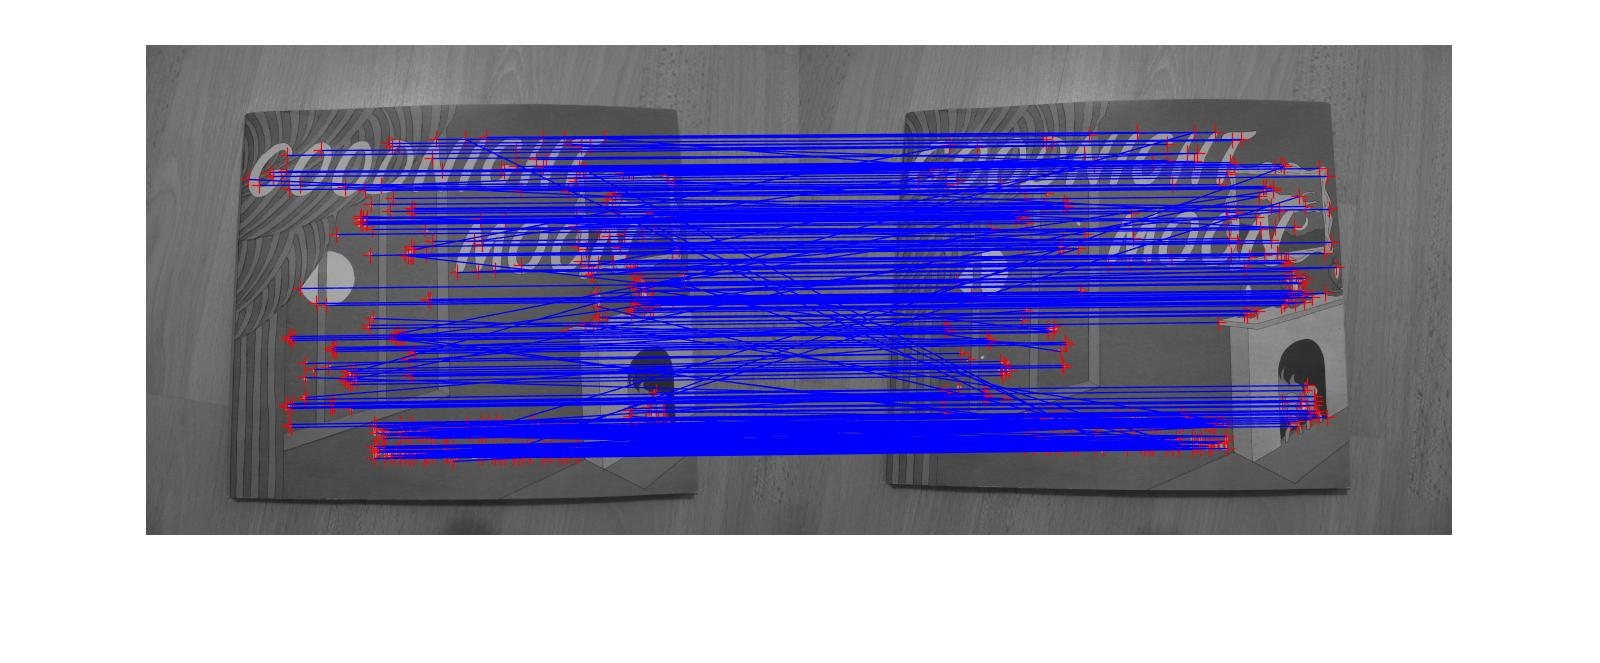
\includegraphics[width=0.9\textwidth]{22.jpg}
	\caption{ one-way nearest neighbors match}
	\label{fig1}
\end{figure}
\begin{figure}[ht]
	\centering
	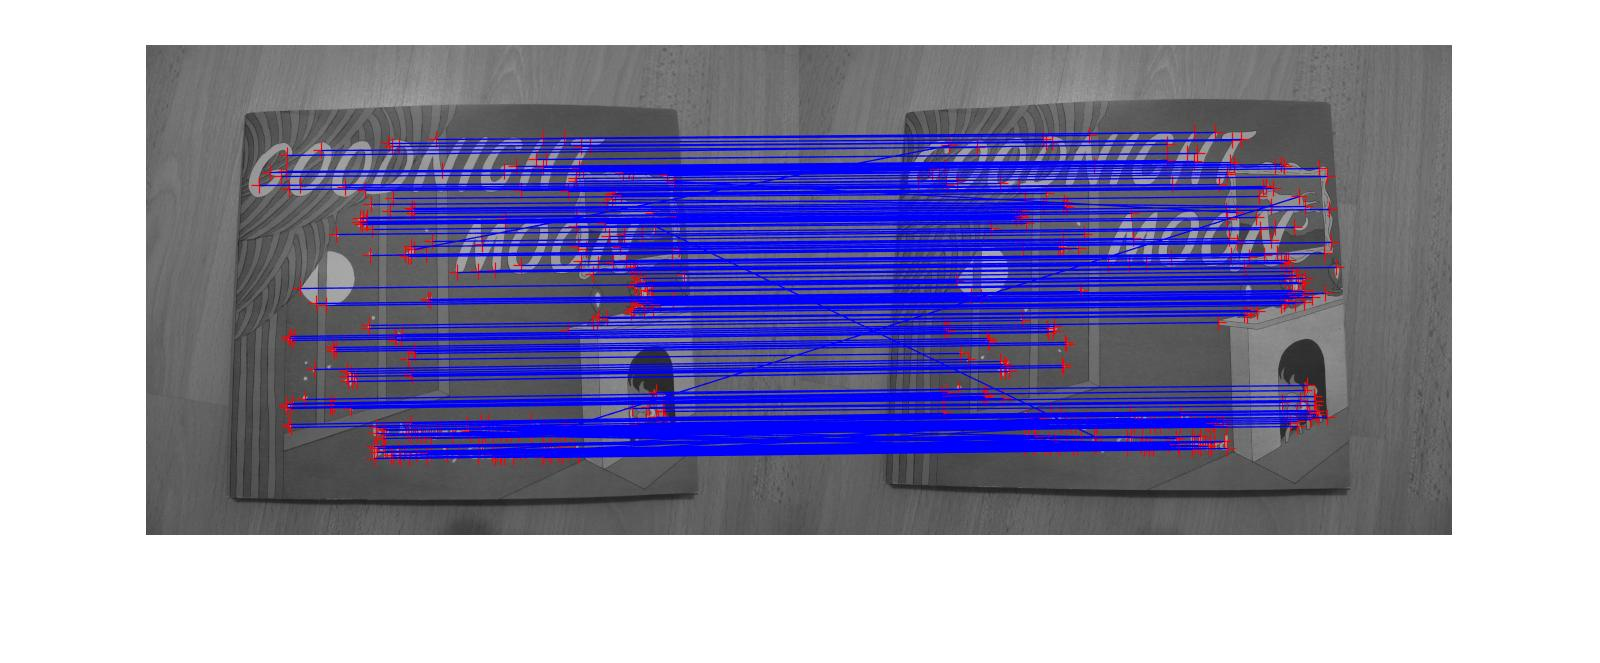
\includegraphics[width=0.9\textwidth]{23.jpg}
	\caption{Mutual nearest neighbors }
	\label{fig1}
\end{figure}
\begin{figure}[ht]
	\centering
	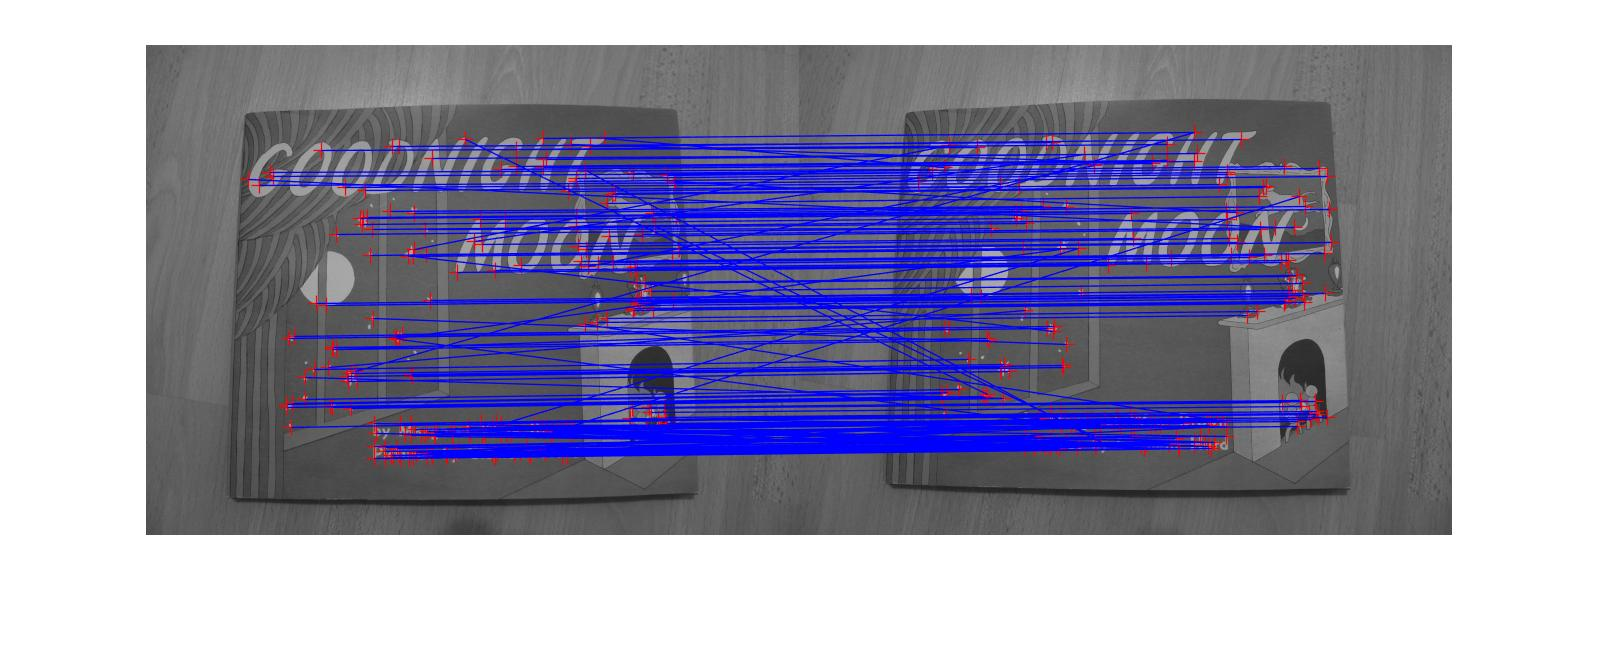
\includegraphics[width=0.9\textwidth]{24.jpg}
	\caption{Ratio}
	\label{fig1}
\end{figure}
\vspace{5mm}

As can be seen the mutual nearest neighbors algorithm yields the best results. The Ratio algorithm performs slightly better than the one way algorithm. But it also eliminates a lot of points. 




\end{document}